\chapter{3D Prototype Silicon Sensors}

The silicon pixels of the LHC are exposed to large amounts of radiation.  The next phase of the LHC (called High Luminosity LHC) will see an order of magnitude higher in the luminosity corresponding to approximately $10^{35} cm ^{-2}s^{-1}$~\cite{SuperLHC}. This luminosity means that the inner tracker will receive a radiation fluence of around $10^{16}n_{eq}/cm^2$.  This is problematic since the current planar silicon detectors only function with a max fluence of approximately $10^{15}n_{eq}/cm^2$.  3D silicon detectors are one of the ways that may provide the necessary radiation tolerance for the next phase of the LHC.

\section{3D Sensors}

Silicon detectors are typically fabricated with planer structures on the material surfaces.  The voltages needed to deplete the detector bulk are typically on the order of tens of volts.  The drift paths are also comparable to the thickness of the bulk~\cite{3dsilicon}. In a 3D detector there are vertical cylindrical electrodes that go through the entire wafer thickness. An example diagram of the processes in a planer and 3D detector is shown in Figure~\ref{fig:operations_3d}~\cite{5734879}. The main reason that 3D detectors have better radiation hardness compared to planer detectors is that there is a much shorter distance between the electrodes.  This is also independent of the thickness of the substrate.  


%%%%%%%%%%%%%%%%%%%%%%%
\begin{figure}[htb!]
\begin{center}
\centerline{
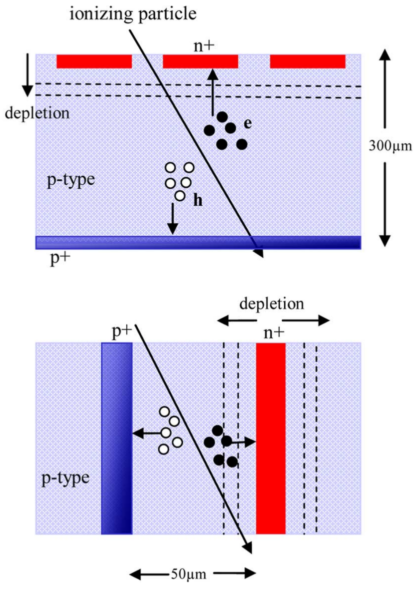
\includegraphics[width=0.45\textwidth]{3D/processes.pdf}
%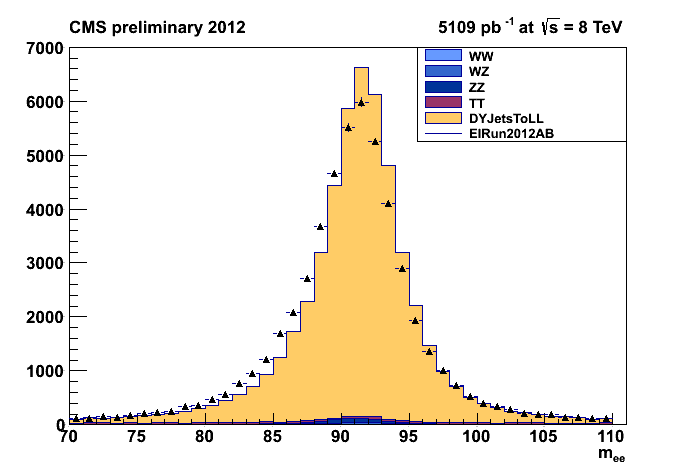
\includegraphics[width=0.45\textwidth]{plots/stdCandle_ElRun2012.png}
%\includegraphics[width=0.45\textwidth]{plots//tmva_massZll.eps}
}
\caption{Operations of planar and 3D detectors are depicted.~\cite{5734879} }
\label{fig:operations_3d}
\end{center}
\end{figure}
%%%%%%%%%%%%%%%%%%%%%%%

There are a variety of different configurations that 3D sensors can use~\cite{3dsilicon}.  The configurations that have been fabricated and are used in the following tests can be seen in Figure~\ref{fig:configuration_3d}. The fabrication was done by SINTEF and one sensor has four readout columns (4E) and the other has 2 (2E) for each CMS pixel that is sized 100 $\mu m$ by 150 $\mu m$.  The distances between each center of the readouts is 62.5 $\mu m$ for the 2E and 45 $\mu m$ for the 4E sensors~\cite{5556029}.


%%%%%%%%%%%%%%%%%%%%%%%
\begin{figure}[htb!]
\begin{center}
\centerline{
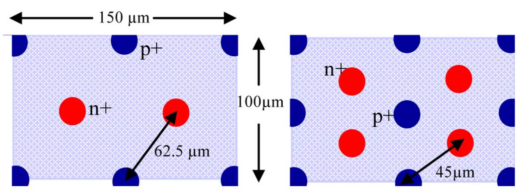
\includegraphics[width=0.75\textwidth]{3D/configuration.pdf}
%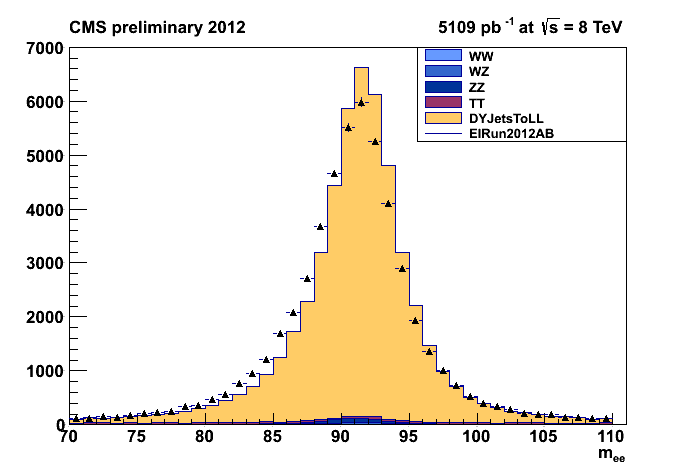
\includegraphics[width=0.45\textwidth]{plots/stdCandle_ElRun2012.png}
%\includegraphics[width=0.45\textwidth]{plots//tmva_massZll.eps}
}
\caption{Sketch of arrangement of columnar electrodes in CMS pixel sensors of
2E type (left) and 4E type(right).~\cite{5734879} }
\label{fig:configuration_3d}
\end{center}
\end{figure}
%%%%%%%%%%%%%%%%%%%%%%%

The fabricated sensors are tested both on the wafer and also after they have been connected to a 40 MhZ CMS pixel readout chip (ROC) through bump-bonds.  Each ROC has 4160 pixels that are organized in a matrix of 52 columns by 80 rows. The characterization of the I-V properties of the 3D pixel sensors can be seen in Figure~\ref{fig:IV_ba}. After the wire bonding, the leakage current drops off for all the sensors tested.  This is because when the sensors were tested on the wafers, only a temporary metal layer was used to connect the columns.  This allowed the entire chip to be tested at once, but led to extra leakage current as can be seen in Figure~\ref{fig:IV_ba}.

%%%%%%%%%%%%%%%%%%%%%%%
\begin{figure}[htb!]
\begin{center}
\centerline{
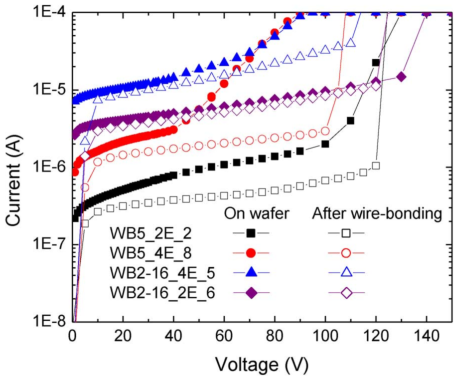
\includegraphics[width=0.75\textwidth]{3D/IV_ba.pdf}
%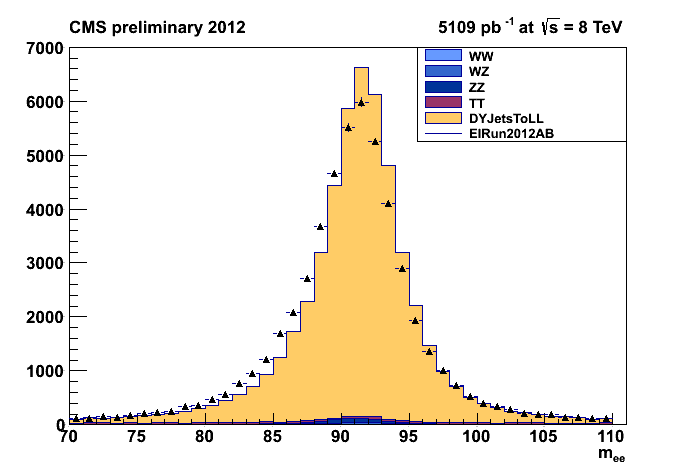
\includegraphics[width=0.45\textwidth]{plots/stdCandle_ElRun2012.png}
%\includegraphics[width=0.45\textwidth]{plots//tmva_massZll.eps}
}
\caption{I-V characteristics of four 3D CMS pixel sensors with different combinations of substrate thickness and electrode configuration as measured at wafer level and after wire-bonding. The convention used in naming is “wafer\_electrode\_configuration\_sensor number”.~\cite{5734879} }
\label{fig:IV_ba}
\end{center}
\end{figure}
%%%%%%%%%%%%%%%%%%%%%%%


\section{Threshold and Noise Measurements}

A scan of the threshold of every pixel is done by injecting an internal charge (VCAL) and then looking at the response versus how much charge was deposited. One VCAL unit corresponds to 65.5 electrons. The ideal curve would be a step function from 0 to 1. But because some of the injected charge below the threshold is not detected, and some of it above the threshold is detected there is a noise component. This noise is the width of the curve.  The efficiency curve is called an S-curve.  This corresponds to the convolution of the ideal step function and the Gaussian pixel noise distribution.

The threshold is the value of charge that corresponds to an efficiency of 0.5 in the S-curve.  The equivalent noise charge (ENC) of the pixel is given below.
\begin{equation} ENC = \dfrac{1}{\sqrt{2\pi}}\dfrac{1}{s} \end{equation}

In this equation, s is the slope of the S-curve at an efficiency of 0.5. The distribution of both the noise and thresholds of the individual pixels make up a Gaussian distribution, which in turn give the threshold and noise of the entire chip. Figure ~\ref{fig:eff_3D} shows the efficiency versus VCAL curves for two pixels, one on the edge and one in the center. Similarly Figure~\ref{fig:noise} shows the map of the noise for each pixel in the rows and columns as they are laid out on the entire sensor.  Also shown is the Gaussian fit for the noise on these pixels.


%%%%%%%%%%%%%%%%%%%%%%%
\begin{figure}[htb!]
\begin{center}
\centerline{
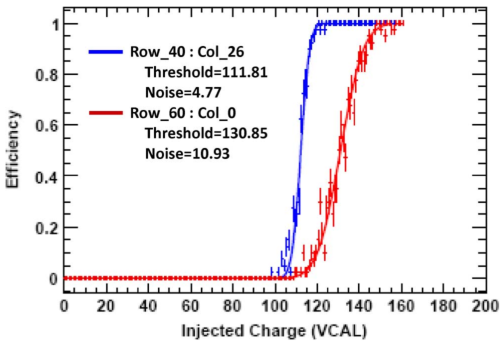
\includegraphics[width=0.55\textwidth]{3D/efficiency.pdf}
}
\caption{S-curves of an edge pixel and a regular pixel in the sensor WB5\_2E\_2
at a reverse bias of 40 V. The threshold and noise values are in VCAL units.~\cite{5734879} }
\label{fig:eff_3D}
\end{center}
\end{figure}
%%%%%%%%%%%%%%%%%%%%%%%

%%%%%%%%%%%%%%%%%%%%%%%
\begin{figure}[htb!]
\begin{center}
\centerline{
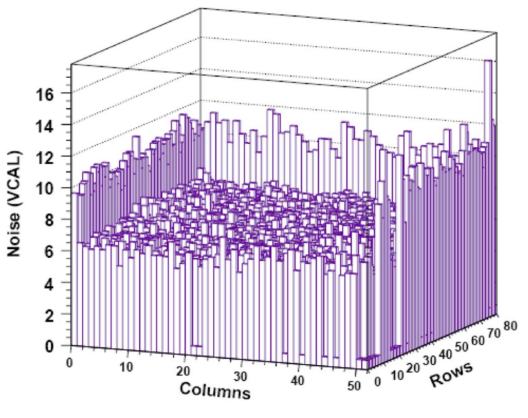
\includegraphics[width=0.45\textwidth]{3D/map.pdf}
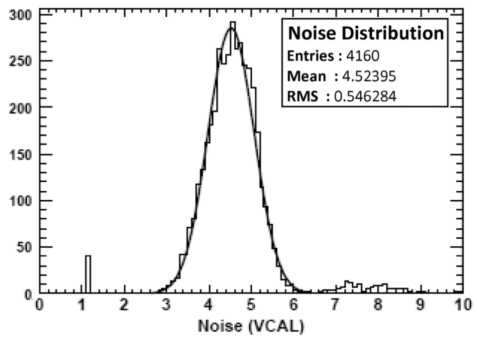
\includegraphics[width=0.45\textwidth]{3D/noise.pdf}
}
\caption{Noise map of the WB5\_2E\_2 chip at a reverse bias of 40 V (left). Gaussian noise distribution of the WB5\_2E\_2 chip at a reverse bias of 40 V (right). ~\cite{5734879} }
\label{fig:noise}
\end{center}
\end{figure}
%%%%%%%%%%%%%%%%%%%%%%%

In addition to measuring the noise performance at just one bias voltage, this has also been done for a range of voltages.  This can be seen in Figure~\ref{fig:bias}. We see that the noise decreases for bias voltages up to 40 V, but beyond this the noise is essentially constant. We also get that the minimum noise for the 2E sensors is approximately 300 electrons and around 450 electrons for the 4E sensors. The 4E sensors have a higher noise compared with the 2E sensors because there is a smaller separation between the electrodes.  This smaller separation is also why both of the 3D detector configurations have higher noise than planer pixel detectors.



%%%%%%%%%%%%%%%%%%%%%%%
\begin{figure}[htb!]
\begin{center}
\centerline{
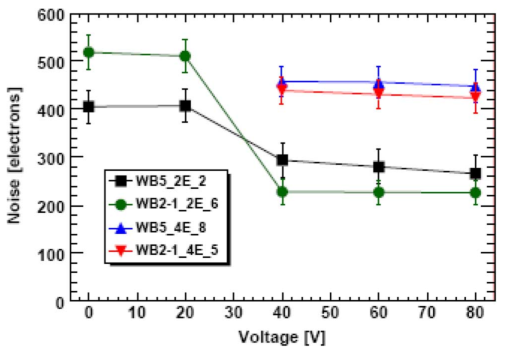
\includegraphics[width=0.65\textwidth]{3D/bias.pdf}
}
\caption{Noise as a function of reverse bias voltage for the four sensors featuring different substrate thickness and electrode configuration.~\cite{5734879} }
\label{fig:bias}
\end{center}
\end{figure}
%%%%%%%%%%%%%%%%%%%%%%%

For the threshold, there is a trimming algorithm that is done to correct variations between pixels and to unify the individual pixel thresholds to the lowest value~\cite{5734879}.  This is needed to improve the position resolution of the detector. Figure~\ref{fig:threshold} shows both the normal threshold measurements and the same measurements using trimming.


%%%%%%%%%%%%%%%%%%%%%%%
\begin{figure}[htb!]
\begin{center}
\centerline{
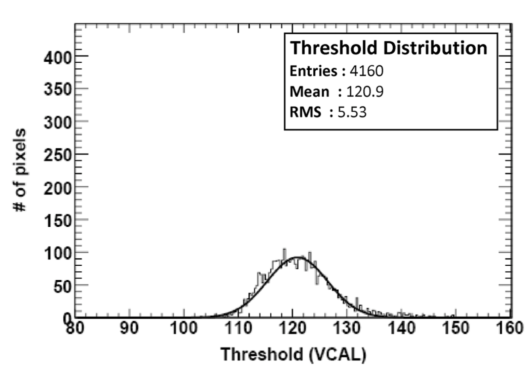
\includegraphics[width=0.45\textwidth]{3D/threshold1.pdf}
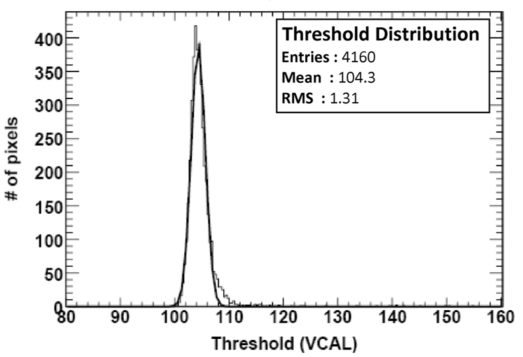
\includegraphics[width=0.45\textwidth]{3D/threshold2.pdf}
}
\caption{Threshold distribution of the WB2-16\_2E\_6 chip at a reverse bias of
40 V before trimming (right) and after trimming (left).~\cite{5734879} }
\label{fig:threshold}
\end{center}
\end{figure}
%%%%%%%%%%%%%%%%%%%%%%%

For the WB2-16\_2E\_6 module with reverse bias voltage of 40 V, the threshold is 7919 $\pm$ 362 electrons before trimming and 6832 $\pm$ 86 electrons after trimming. The other modules have similar performance. Compared with the FPIX detector (and BPIX) which has a threshold of 2870 $\pm$ 220 electrons (2940 $\pm$ 80), the 3D detector display higher thresholds~\cite{CMSpixel}.

Since these studies have been performed, there have been a number of improvements particularly in fabrication of the 3D sensors and the ability to fabricate them without any support structure.  With additional improvements that have also been made in the trimming algorithms, 3D pixel detectors are proving to be very promising for the future pixel upgrade to the High Luminosity LHC.  
